% Requires in your main LaTeX preamble:
% \usepackage{graphicx}
% \usepackage{float}
% \usepackage{caption}
%
% Optional but recommended for top-aligning float pages:
% \makeatletter
% \setlength{\@fptop}{0pt}
% \setlength{\@fpsep}{8pt}
% \setlength{\@fpbot}{0pt plus 1fil}
% \makeatother

\clearpage
\begin{figure}[p]
    \centering
    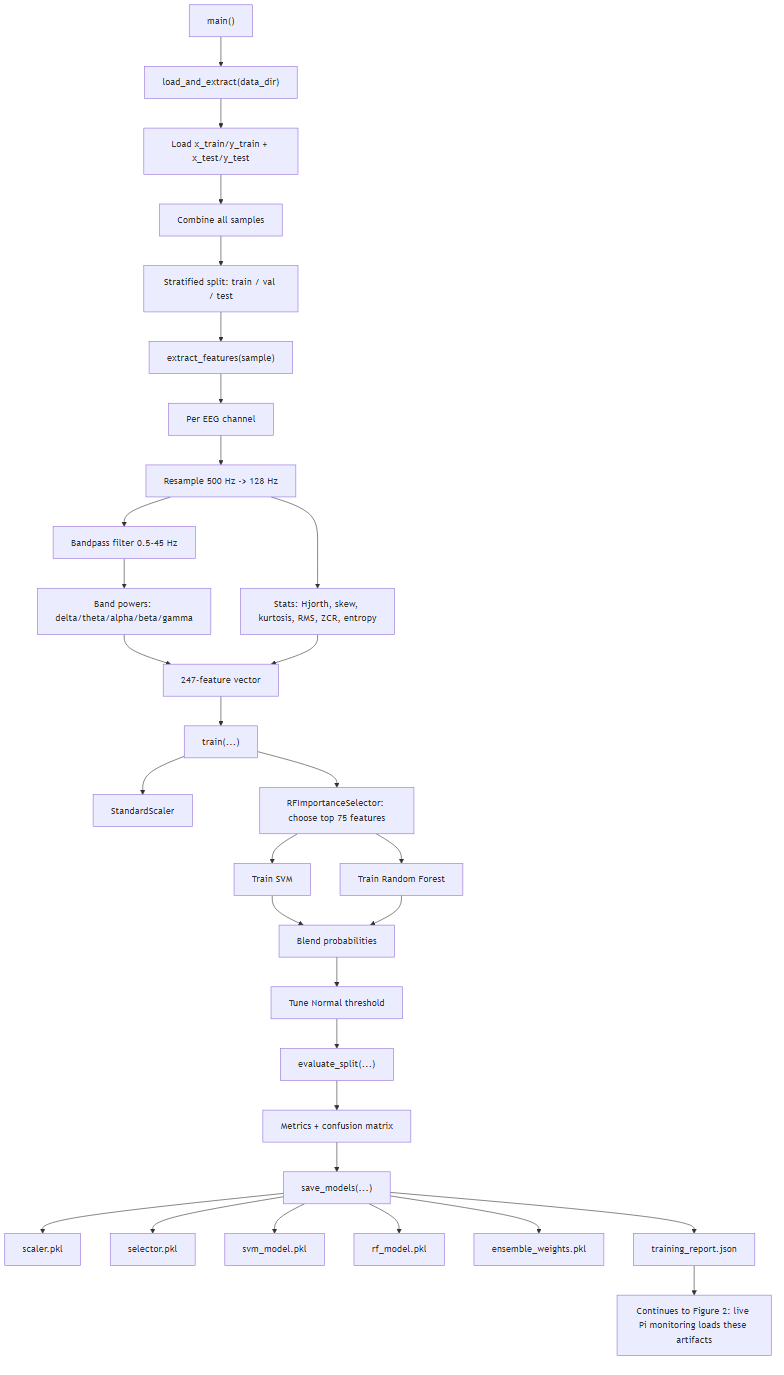
\includegraphics[
        width=0.95\textwidth,
        height=0.82\textheight,
        keepaspectratio
    ]{docs/flowchart_part_1_training.png}
    \caption{NeuroWatch training pipeline and saved model artifacts.}
    \label{fig:neurowatch-training-flow}
\end{figure}

\clearpage
\begin{figure}[p]
    \centering

    \includegraphics[
        width=0.95\textwidth,
        height=0.39\textheight,
        keepaspectratio
    ]{images/docs/flowchart_part_2_runtime_hardware.png}

    \caption*{(a) Live Raspberry Pi monitoring pipeline and hardware outputs.}

    \vspace{0.8em}

    \includegraphics[
        width=0.95\textwidth,
        height=0.39\textheight,
        keepaspectratio
    ]{images/docs/flowchart_part_3_dashboard.png}

    \caption*{(b) Runtime JSON outputs consumed by the clinician dashboard and patient mobile UI.}

    \caption{Live monitoring hardware outputs and dashboard integration.}
    \label{fig:neurowatch-runtime-dashboard-flow}
\end{figure}
\clearpage
